\documentclass{article}
\usepackage[margin=1in]{geometry}
\usepackage{datetime}
\usepackage{qcircuit}
\usepackage{amsmath}
\usepackage{pgfplots}
\pgfplotsset{compat=1.18}
\usepackage[utf8]{inputenc}
\begin{document}
\begin{center}
    {\LARGE \textbf{mimiQ++ Report}} \\
    \large \today \quad \currenttime
\end{center}
\hrule
\vspace{1cm}
\clearpage
\section*{Quantum Circuit}
\begin{figure}[htbp]
    \centering
    \[
    \Qcircuit @C=1em @R=.7em {
\lstick{q0} & \gate{U(0.3,0.2,0.1)} & \qw & \ctrl{1} & \gate{H} & \meter & \qw & \qw & \qw & \qw & \qw & \\ 
\lstick{q1} & \gate{H} & \ctrl{1} & \gate{X} & \qw & \qw \cwx & \meter & \qw & \qw & \qw & \qw & \\ 
\lstick{q2} & \qw & \gate{X} & \qw & \qw & \qw \cwx & \qw \cwx & \gate{X} & \gate{Z} & \meter & \qw & \\ 
\lstick{c0} & \cw & \cw & \cw & \cw & \cw \cwx & \cw \cwx & \cw \cwx & \control \cw \cwx & \cw \cwx & \cw & \\ 
\lstick{c1} & \cw & \cw & \cw & \cw & \cw & \cw \cwx & \control \cw \cwx & \cw & \cw \cwx & \cw & \\ 
\lstick{c2} & \cw & \cw & \cw & \cw & \cw & \cw & \cw & \cw & \cw \cwx & \cw & \\ 
\\ 
\\ 
}
\]
\caption{quantum teleportation 1}
\end{figure}
\begin{center}
    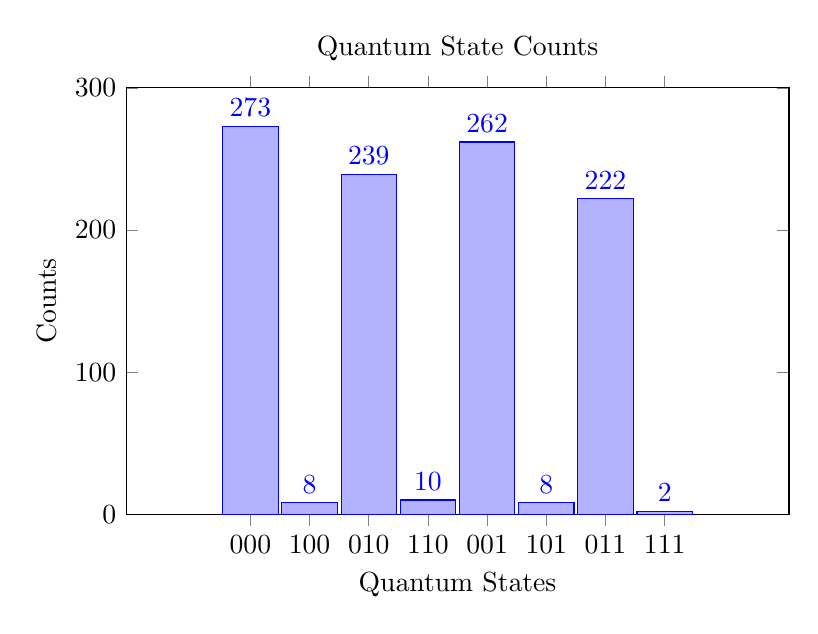
\begin{tikzpicture}
        \begin{axis}[
            ybar,
            symbolic x coords={000, 100, 010, 110, 001, 101, 011, 111},
            xtick=data,
            xlabel={Quantum States},
            ylabel={Counts},
            ymin=0,
            bar width=20pt,
            width=10cm,
            height=7cm,
            nodes near coords,
            nodes near coords align={vertical},
            enlarge x limits=0.3,
            title={Quantum State Counts}
        ]
        \addplot coordinates {(000,273) (100,8) (010,239) (110,10) (001,262) (101,8) (011,222) (111,2) };
        \end{axis}
    \end{tikzpicture}
\end{center}


the OpenQASM 2.0 code for the above qircuit is: 


\begin{verbatim}
OPENQASM 2.0;
include "qelib1.inc";
qreg q[3];
creg c[3];
u(0.300000,0.200000,0.100000) q[0];
h q[1];
cx q[1], q[2];
cx q[0], q[1];
h q[0];
measure q[0] -> c[0];
measure q[1] -> c[1];
if ( c == 2) x q[2];
if ( c == 1) z q[2];
measure q[2] -> c[2];
\end{verbatim}
\clearpage
\section*{Quantum Circuit}
\begin{figure}[htbp]
    \centering
    \[
    \Qcircuit @C=1em @R=.7em {
\lstick{q0} & \gate{U(6.28,0.408,2.22)} & \qw & \ctrl{1} & \gate{H} & \meter & \qw & \qw & \qw &  \qw & \\
\lstick{q1} & \gate{H} & \ctrl{1} & \gate{X} & \qw & \qw \cwx & \meter & \qw & \qw &  \qw & \\
\lstick{q2} & \qw & \gate{X} & \qw & \qw & \qw \cwx & \qw \cwx & \gate{X} & \gate{Z} &  \qw & \\
\lstick{c0} & \cw & \cw & \cw & \cw & \cw \cwx & \cw \cwx & \cw \cwx & \control \cw \cwx &  \cw & \\
\lstick{c1} & \cw & \cw & \cw & \cw & \cw & \cw \cwx & \control \cw \cwx & \cw &  \cw & \\
\lstick{c2} & \cw & \cw & \cw & \cw & \cw & \cw & \cw & \cw &  \cw & \\
\\ 
\\ 
\lstick{q0} & \qw & \qw & \qw & \\ 
\lstick{q1} & \qw & \qw & \qw & \\ 
\lstick{q2} & \gate{U(-6.28,-2.22,-0.408)} & \meter & \qw & \\ 
\lstick{c0} & \cw & \cw \cwx & \cw & \\ 
\lstick{c1} & \cw & \cw \cwx & \cw & \\ 
\lstick{c2} & \cw & \cw \cwx & \cw & \\ 
\\ 
\\ 
}
\]
\caption{quantum teleportation ibm}
\end{figure}
\begin{center}
    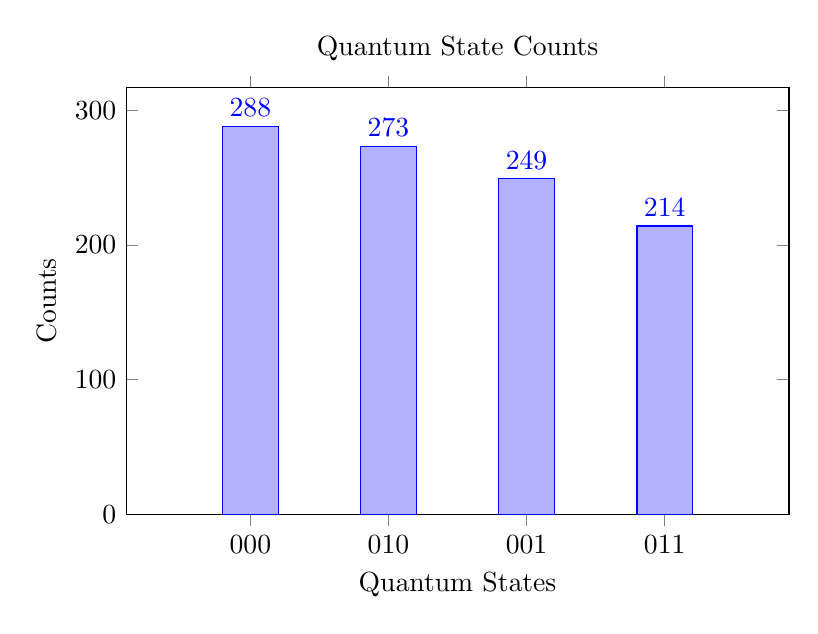
\begin{tikzpicture}
        \begin{axis}[
            ybar,
            symbolic x coords={000, 010, 001, 011},
            xtick=data,
            xlabel={Quantum States},
            ylabel={Counts},
            ymin=0,
            bar width=20pt,
            width=10cm,
            height=7cm,
            nodes near coords,
            nodes near coords align={vertical},
            enlarge x limits=0.3,
            title={Quantum State Counts}
        ]
        \addplot coordinates {(000,288) (010,273) (001,249) (011,214) };
        \end{axis}
    \end{tikzpicture}
\end{center}


the OpenQASM 2.0 code for the above qircuit is: 


\begin{verbatim}
qreg q[3];
creg c[3];
u(6.280000,0.408000,2.220000) q[0];
h q[1];
cx q[1], q[2];
cx q[0], q[1];
h q[0];
measure q[0] -> c[0];
measure q[1] -> c[1];
if ( c == 2) x q[2];
if ( c == 1) z q[2];
u(-6.280000,-2.220000,-0.408000) q[2];
measure q[2] -> c[2];
\end{verbatim}
\clearpage
\section*{Quantum Circuit}
\begin{figure}[htbp]
    \centering
    \[
    \Qcircuit @C=1em @R=.7em {
\lstick{q0} & \gate{X} & \meter & \gate{X} & \gate{H} & \ctrl{1} & \gate{Z} & \gate{X} & \ctrl{1} & \gate{H} & \meter & \qw & \qw & \\ 
\lstick{q1} & \qw & \qw \cwx & \qw & \qw & \gate{X} & \qw \cwx & \qw \cwx & \gate{X} & \qw & \qw \cwx & \meter & \qw & \\ 
\lstick{c0} & \cw & \cw \cwx & \cw & \cw & \cw & \cw \cwx & \control \cw \cwx & \cw & \cw & \cw \cwx & \cw \cwx & \cw & \\ 
\lstick{c1} & \cw & \cw \cwx & \cw & \cw & \cw & \control \cw \cwx & \cw & \cw & \cw & \cw \cwx & \cw \cwx & \cw & \\ 
\lstick{c2} & \cw & \cw & \cw & \cw & \cw & \cw & \cw & \cw & \cw & \cw \cwx & \cw \cwx & \cw & \\ 
\lstick{c3} & \cw & \cw & \cw & \cw & \cw & \cw & \cw & \cw & \cw & \cw \cwx & \cw & \cw & \\ 
\\ 
\\ 
}
\]
\caption{superdense coding}
\end{figure}
\begin{center}
    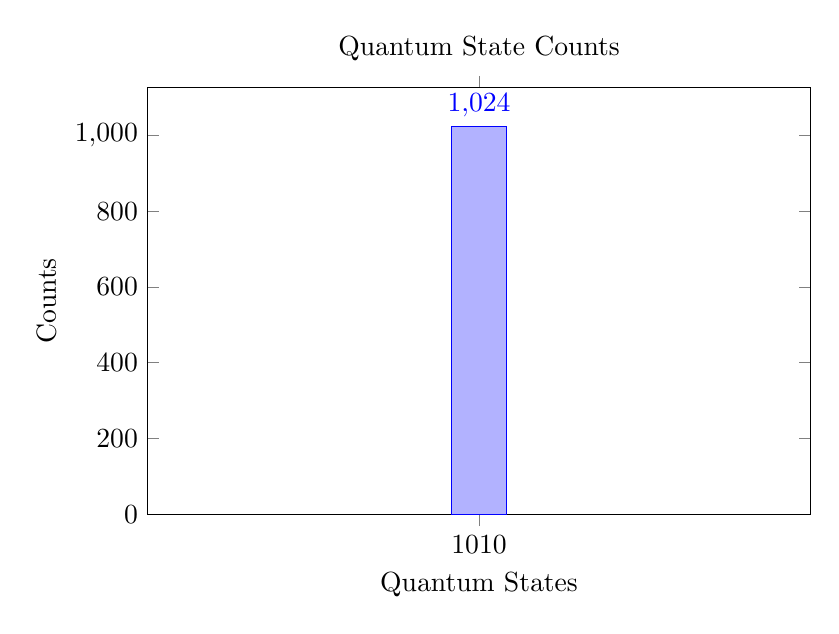
\begin{tikzpicture}
        \begin{axis}[
            ybar,
            symbolic x coords={1010},
            xtick=data,
            xlabel={Quantum States},
            ylabel={Counts},
            ymin=0,
            bar width=20pt,
            width=10cm,
            height=7cm,
            nodes near coords,
            nodes near coords align={vertical},
            enlarge x limits=0.3,
            title={Quantum State Counts}
        ]
        \addplot coordinates {(1010,1024) };
        \end{axis}
    \end{tikzpicture}
\end{center}


the OpenQASM 2.0 code for the above qircuit is: 


\begin{verbatim}
qreg q[2];
creg c[4];
x q[0];
measure q[0] -> c[1];
x q[0];
h q[0];
cx q[0], q[1];
if ( c == 2) z q[0];
if ( c == 1) x q[0];
cx q[0], q[1];
h q[0];
measure q[0] -> c[3];
measure q[1] -> c[2];
\end{verbatim}
\clearpage
\section*{Quantum Circuit}
\begin{figure}[htbp]
    \centering
    \[
    \Qcircuit @C=1em @R=.7em {
\lstick{q0} & \gate{H} & \qw & \qw & \qw & \qw & \ctrl{1} & \gate{Z} & \gate{X} & \ctrl{1} & \gate{H} & \meter & \qw & \qw & \\ 
\lstick{q1} & \qw & \qw & \qw & \qw & \qw & \gate{X} & \qw \cwx & \qw \cwx & \gate{X} & \qw & \qw \cwx & \meter & \qw & \\ 
\lstick{q2} & \gate{H} & \meter & \gate{X} & \gate{H} & \meter & \qw & \qw \cwx & \qw \cwx & \qw & \qw & \qw \cwx & \qw \cwx & \qw & \\ 
\lstick{c0} & \cw & \cw \cwx & \control \cw \cwx & \cw & \cw \cwx & \cw & \cw \cwx & \control \cw \cwx & \cw & \cw & \cw \cwx & \cw \cwx & \cw & \\ 
\lstick{c1} & \cw & \cw & \cw & \cw & \cw \cwx & \cw & \control \cw \cwx & \cw & \cw & \cw & \cw \cwx & \cw \cwx & \cw & \\ 
\lstick{c2} & \cw & \cw & \cw & \cw & \cw & \cw & \cw & \cw & \cw & \cw & \cw \cwx & \cw \cwx & \cw & \\ 
\lstick{c3} & \cw & \cw & \cw & \cw & \cw & \cw & \cw & \cw & \cw & \cw & \cw \cwx & \cw & \cw & \\ 
\\ 
\\ 
}
\]
\caption{superdense coding - random}
\end{figure}
\begin{center}
    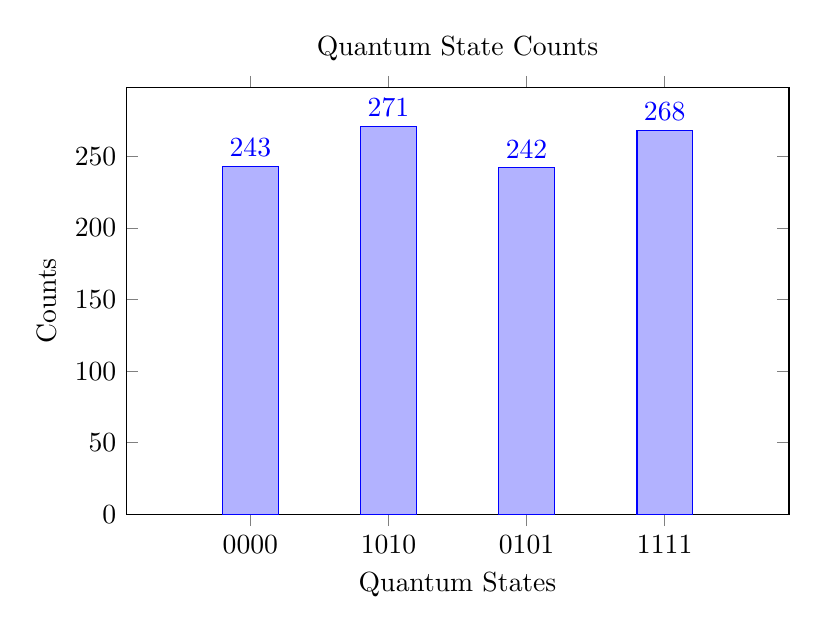
\begin{tikzpicture}
        \begin{axis}[
            ybar,
            symbolic x coords={0000, 1010, 0101, 1111},
            xtick=data,
            xlabel={Quantum States},
            ylabel={Counts},
            ymin=0,
            bar width=20pt,
            width=10cm,
            height=7cm,
            nodes near coords,
            nodes near coords align={vertical},
            enlarge x limits=0.3,
            title={Quantum State Counts}
        ]
        \addplot coordinates {(0000,243) (1010,271) (0101,242) (1111,268) };
        \end{axis}
    \end{tikzpicture}
\end{center}


the OpenQASM 2.0 code for the above qircuit is: 


\begin{verbatim}
qreg q[3];
creg c[4];
h q[2];
measure q[2] -> c[0];
if ( c == 1) x q[2];
h q[2];
measure q[2] -> c[1];
h q[0];
cx q[0], q[1];
if ( c == 2) z q[0];
if ( c == 1) x q[0];
cx q[0], q[1];
h q[0];
measure q[0] -> c[3];
measure q[1] -> c[2];
\end{verbatim}
\clearpage
\section*{Quantum Circuit}
\begin{figure}[htbp]
    \centering
    \[
    \Qcircuit @C=1em @R=.7em {
\lstick{q0} & \qw & \qw & \qw & \gate{X} & \qw & \qw & \qw & \gate{H} & \qw & \qw & \qw & \qw & \qw & \qw &  \qw & \\
\lstick{q1} & \gate{H} & \meter & \gate{X} & \qw \cwx & \gate{H} & \meter & \gate{X} & \qw \cwx & \gate{H} & \meter & \gate{X} & \gate{H} & \meter & \gate{X} &  \qw & \\
\lstick{c0} & \cw & \cw \cwx & \control \cw \cwx & \control \cw \cwx & \cw & \cw \cwx & \cw \cwx & \cw \cwx & \cw & \cw \cwx & \cw \cwx & \cw & \cw \cwx & \cw \cwx &  \cw & \\
\lstick{c1} & \cw & \cw & \cw & \cw & \cw & \cw \cwx & \control \cw \cwx & \control \cw \cwx & \cw & \cw \cwx & \cw \cwx & \cw & \cw \cwx & \cw \cwx &  \cw & \\
\lstick{c2} & \cw & \cw & \cw & \cw & \cw & \cw & \cw & \cw & \cw & \cw \cwx & \cw \cwx & \cw & \cw \cwx & \cw \cwx &  \cw & \\
\lstick{c3} & \cw & \cw & \cw & \cw & \cw & \cw & \cw & \cw & \cw & \cw \cwx & \cw \cwx & \cw & \cw \cwx & \cw \cwx &  \cw & \\
\lstick{c4} & \cw & \cw & \cw & \cw & \cw & \cw & \cw & \cw & \cw & \cw \cwx & \control \cw \cwx & \cw & \cw \cwx & \cw \cwx &  \cw & \\
\lstick{c5} & \cw & \cw & \cw & \cw & \cw & \cw & \cw & \cw & \cw & \cw & \cw & \cw & \cw \cwx & \control \cw \cwx &  \cw & \\
\\ 
\\ 
\lstick{q0} & \gate{X} & \qw & \qw & \qw & \gate{H} & \qw & \qw & \meter & \qw & \\ 
\lstick{q1} & \qw \cwx & \gate{H} & \meter & \gate{X} & \qw \cwx & \gate{H} & \meter & \qw \cwx & \qw & \\ 
\lstick{c0} & \cw \cwx & \cw & \cw \cwx & \cw \cwx & \cw \cwx & \cw & \cw \cwx & \cw \cwx & \cw & \\ 
\lstick{c1} & \cw \cwx & \cw & \cw \cwx & \cw \cwx & \cw \cwx & \cw & \cw \cwx & \cw \cwx & \cw & \\ 
\lstick{c2} & \cw \cwx & \cw & \cw \cwx & \cw \cwx & \cw \cwx & \cw & \cw \cwx & \cw \cwx & \cw & \\ 
\lstick{c3} & \cw \cwx & \cw & \cw \cwx & \cw \cwx & \cw \cwx & \cw & \cw & \cw \cwx & \cw & \\ 
\lstick{c4} & \cw \cwx & \cw & \cw \cwx & \cw \cwx & \cw \cwx & \cw & \cw & \cw & \cw & \\ 
\lstick{c5} & \control \cw \cwx & \cw & \cw \cwx & \control \cw \cwx & \control \cw \cwx & \cw & \cw & \cw & \cw & \\ 
\\ 
\\ 
}
\]
\caption{BB84-ptcl QKD}
\end{figure}
Resultant key: 01001111110100010000111010011101001111001101100100

\clearpage
\section*{Quantum Circuit}
\begin{figure}[htbp]
    \centering
    \[
    \Qcircuit @C=1em @R=.7em {
\lstick{q0} & \gate{H} & \gate{X} & \ctrl{2} & \gate{X} & \gate{H} & \gate{X} & \qw & \ctrl{2} & \gate{X} & \gate{H} & \gate{X} & \qw & \ctrl{2} & \gate{X} &  \qw & \\
\lstick{q1} & \gate{H} & \qw & \ctrl{1} & \gate{H} & \gate{X} & \qw & \qw & \ctrl{1} & \gate{X} & \gate{H} & \qw & \qw & \ctrl{1} & \gate{H} &  \qw & \\
\lstick{q2} & \gate{H} & \gate{H} & \gate{X} & \gate{H} & \gate{H} & \gate{X} & \gate{H} & \gate{X} & \gate{H} & \gate{X} & \gate{H} & \gate{H} & \gate{X} & \gate{H} &  \qw & \\
\lstick{c0} & \cw & \cw & \cw & \cw & \cw & \cw & \cw & \cw & \cw & \cw & \cw & \cw & \cw & \cw &  \cw & \\
\lstick{c1} & \cw & \cw & \cw & \cw & \cw & \cw & \cw & \cw & \cw & \cw & \cw & \cw & \cw & \cw &  \cw & \\
\lstick{c2} & \cw & \cw & \cw & \cw & \cw & \cw & \cw & \cw & \cw & \cw & \cw & \cw & \cw & \cw &  \cw & \\
\\ 
\\ 
\lstick{q0} & \gate{H} & \gate{X} & \qw & \ctrl{2} & \gate{X} & \gate{H} & \qw & \meter & \qw & \qw & \qw & \\ 
\lstick{q1} & \gate{X} & \qw & \qw & \ctrl{1} & \gate{X} & \gate{H} & \qw & \qw \cwx & \meter & \qw & \qw & \\ 
\lstick{q2} & \gate{H} & \gate{X} & \gate{H} & \gate{X} & \gate{H} & \gate{X} & \gate{H} & \qw \cwx & \qw \cwx & \meter & \qw & \\ 
\lstick{c0} & \cw & \cw & \cw & \cw & \cw & \cw & \cw & \cw \cwx & \cw \cwx & \cw \cwx & \cw & \\ 
\lstick{c1} & \cw & \cw & \cw & \cw & \cw & \cw & \cw & \cw & \cw \cwx & \cw \cwx & \cw & \\ 
\lstick{c2} & \cw & \cw & \cw & \cw & \cw & \cw & \cw & \cw & \cw & \cw \cwx & \cw & \\ 
\\ 
\\ 
}
\]
\caption{grover}
\end{figure}
\begin{center}
    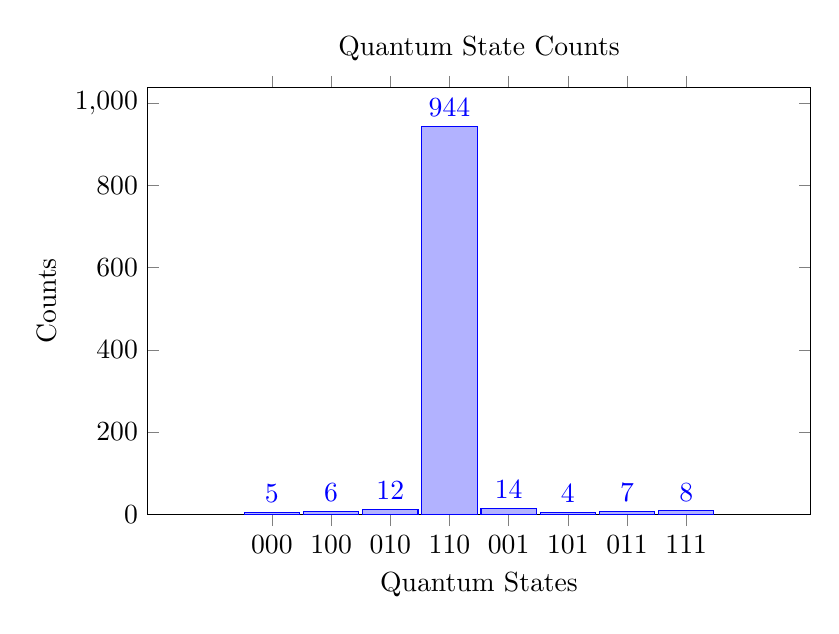
\begin{tikzpicture}
        \begin{axis}[
            ybar,
            symbolic x coords={000, 100, 010, 110, 001, 101, 011, 111},
            xtick=data,
            xlabel={Quantum States},
            ylabel={Counts},
            ymin=0,
            bar width=20pt,
            width=10cm,
            height=7cm,
            nodes near coords,
            nodes near coords align={vertical},
            enlarge x limits=0.3,
            title={Quantum State Counts}
        ]
        \addplot coordinates {(000,5) (100,6) (010,12) (110,944) (001,14) (101,4) (011,7) (111,8) };
        \end{axis}
    \end{tikzpicture}
\end{center}


the OpenQASM 2.0 code for the above qircuit is: 


\begin{verbatim}
qreg q[3];
creg c[3];
h q[2];
h q[1];
h q[0];
x q[0];
h q[2];
ccx q[0], q[1], q[2];
h q[2];
x q[0];
h q[0];
h q[1];
h q[2];
x q[0];
x q[1];
x q[2];
h q[2];
ccx q[0], q[1], q[2];
h q[2];
x q[1];
x q[0];
x q[2];
h q[0];
h q[1];
h q[2];
x q[0];
h q[2];
ccx q[0], q[1], q[2];
h q[2];
x q[0];
h q[0];
h q[1];
h q[2];
x q[0];
x q[1];
x q[2];
h q[2];
ccx q[0], q[1], q[2];
h q[2];
x q[1];
x q[0];
x q[2];
h q[0];
h q[1];
h q[2];
measure q[0] -> c[0];
measure q[1] -> c[1];
measure q[2] -> c[2];
\end{verbatim}
\clearpage
\section*{Quantum Circuit}
\begin{figure}[htbp]
    \centering
    \[
    \Qcircuit @C=1em @R=.7em {
\lstick{q0} & \gate{X} & \ctrl{2} & \ctrl{1} & \qw & \qw & \ctrl{1} & \meter & \qw & \qw & \qw & \qw & \\ 
\lstick{q1} & \qw & \ctrl{1} & \gate{X} & \ctrl{2} & \ctrl{1} & \gate{X} & \qw \cwx & \meter & \qw & \qw & \qw & \\ 
\lstick{q2} & \gate{X} & \gate{X} & \qw & \ctrl{1} & \gate{X} & \qw & \qw \cwx & \qw \cwx & \meter & \qw & \qw & \\ 
\lstick{q3} & \qw & \qw & \qw & \gate{X} & \qw & \qw & \qw \cwx & \qw \cwx & \qw \cwx & \meter & \qw & \\ 
\lstick{c0} & \cw & \cw & \cw & \cw & \cw & \cw & \cw \cwx & \cw \cwx & \cw \cwx & \cw \cwx & \cw & \\ 
\lstick{c1} & \cw & \cw & \cw & \cw & \cw & \cw & \cw & \cw \cwx & \cw \cwx & \cw \cwx & \cw & \\ 
\lstick{c2} & \cw & \cw & \cw & \cw & \cw & \cw & \cw & \cw & \cw \cwx & \cw \cwx & \cw & \\ 
\lstick{c3} & \cw & \cw & \cw & \cw & \cw & \cw & \cw & \cw & \cw & \cw \cwx & \cw & \\ 
\\ 
\\ 
}
\]
\caption{full adder}
\end{figure}
\begin{center}
    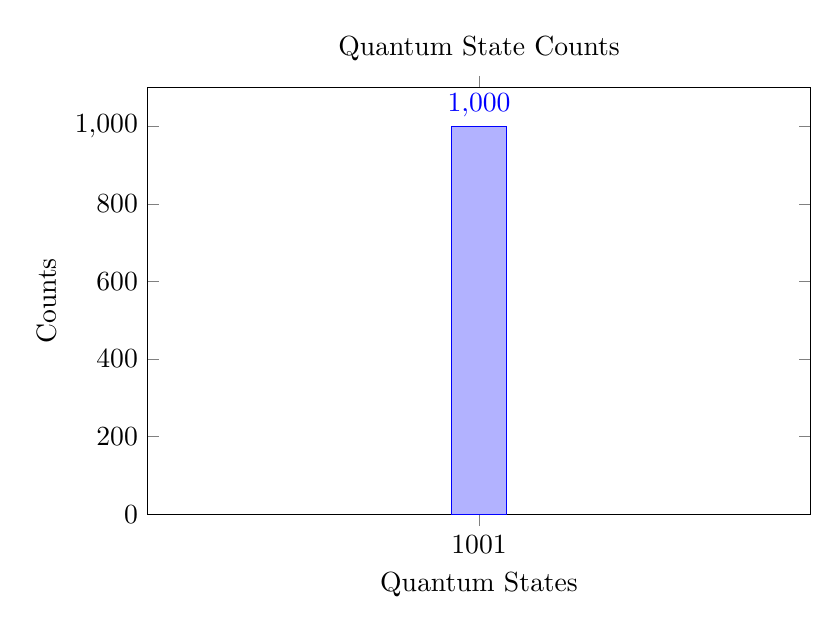
\begin{tikzpicture}
        \begin{axis}[
            ybar,
            symbolic x coords={1001},
            xtick=data,
            xlabel={Quantum States},
            ylabel={Counts},
            ymin=0,
            bar width=20pt,
            width=10cm,
            height=7cm,
            nodes near coords,
            nodes near coords align={vertical},
            enlarge x limits=0.3,
            title={Quantum State Counts}
        ]
        \addplot coordinates {(1001,1000) };
        \end{axis}
    \end{tikzpicture}
\end{center}


the OpenQASM 2.0 code for the above qircuit is: 


\begin{verbatim}
qreg q[4];
creg c[4];
x q[0];
x q[2];
ccx q[0], q[1], q[2];
cx q[0], q[1];
ccx q[1], q[2], q[3];
cx q[1], q[2];
cx q[0], q[1];
measure q[0] -> c[0];
measure q[1] -> c[1];
measure q[2] -> c[2];
measure q[3] -> c[3];
\end{verbatim}
\clearpage
\section*{Quantum Circuit}
\begin{figure}[htbp]
    \centering
    \[
    \Qcircuit @C=1em @R=.7em {
\lstick{q0} & \gate{H} & \qw & \qw & \qw & \qw & \ctrl{2} & \ctrl{2} & \qw & \ctrl{2} & \qw &  \qw & \\
\lstick{q1} & \gate{H} & \ctrl{1} & \qw & \ctrl{1} & \gate{X} & \ctrl{1} & \qw & \qw & \qw & \qw &  \qw & \\
\lstick{q2} & \qw & \gate{X} & \gate{Ry(0.111)} & \gate{X} & \gate{Ry(-0.111)} & \gate{X} & \gate{X} & \gate{Ry(0)} & \gate{X} & \gate{Ry(0)} &  \qw & \\
\lstick{q3} & \qw & \qw & \qw & \qw & \qw & \qw & \qw & \qw & \qw & \qw &  \qw & \\
\lstick{c0} & \cw & \cw & \cw & \cw & \cw & \cw & \cw & \cw & \cw & \cw &  \cw & \\
\lstick{c1} & \cw & \cw & \cw & \cw & \cw & \cw & \cw & \cw & \cw & \cw &  \cw & \\
\lstick{c2} & \cw & \cw & \cw & \cw & \cw & \cw & \cw & \cw & \cw & \cw &  \cw & \\
\lstick{c3} & \cw & \cw & \cw & \cw & \cw & \cw & \cw & \cw & \cw & \cw &  \cw & \\
\\ 
\\ 
\lstick{q0} & \ctrl{2} & \ctrl{2} & \qw & \ctrl{2} & \gate{X} & \ctrl{2} & \ctrl{2} & \qw & \ctrl{2} & \qw & \ctrl{2} &  \qw & \\
\lstick{q1} & \ctrl{1} & \qw & \qw & \qw & \qw & \ctrl{1} & \qw & \qw & \qw & \qw & \ctrl{1} &  \qw & \\
\lstick{q2} & \gate{X} & \gate{X} & \gate{Ry(0)} & \gate{X} & \gate{Ry(0)} & \gate{X} & \gate{X} & \gate{Ry(-1.511)} & \gate{X} & \gate{Ry(1.511)} & \gate{X} &  \qw & \\
\lstick{q3} & \qw & \qw & \qw & \qw & \qw & \qw & \qw & \qw & \qw & \qw & \qw &  \qw & \\
\lstick{c0} & \cw & \cw & \cw & \cw & \cw & \cw & \cw & \cw & \cw & \cw & \cw &  \cw & \\
\lstick{c1} & \cw & \cw & \cw & \cw & \cw & \cw & \cw & \cw & \cw & \cw & \cw &  \cw & \\
\lstick{c2} & \cw & \cw & \cw & \cw & \cw & \cw & \cw & \cw & \cw & \cw & \cw &  \cw & \\
\lstick{c3} & \cw & \cw & \cw & \cw & \cw & \cw & \cw & \cw & \cw & \cw & \cw &  \cw & \\
\\ 
\\ 
\lstick{q0} & \ctrl{2} & \qw & \ctrl{2} & \qw & \ctrl{3} & \qw & \qw & \qw & \qw & \\ 
\lstick{q1} & \qw & \qw & \qw & \qw & \qw & \gate{H} & \meter & \qw & \qw & \\ 
\lstick{q2} & \gate{X} & \gate{Ry(1.511)} & \gate{X} & \gate{Ry(-1.511)} & \qw & \qw & \qw \cwx & \qw & \qw & \\ 
\lstick{q3} & \qw & \qw & \qw & \qw & \gate{X} & \qw & \qw \cwx & \meter & \qw & \\ 
\lstick{c0} & \cw & \cw & \cw & \cw & \cw & \cw & \cw \cwx & \cw \cwx & \cw & \\ 
\lstick{c1} & \cw & \cw & \cw & \cw & \cw & \cw & \cw \cwx & \cw \cwx & \cw & \\ 
\lstick{c2} & \cw & \cw & \cw & \cw & \cw & \cw & \cw & \cw \cwx & \cw & \\ 
\lstick{c3} & \cw & \cw & \cw & \cw & \cw & \cw & \cw & \cw \cwx & \cw & \\ 
\\ 
\\ 
}
\]
\caption{quantum classification}
\end{figure}
\begin{center}
    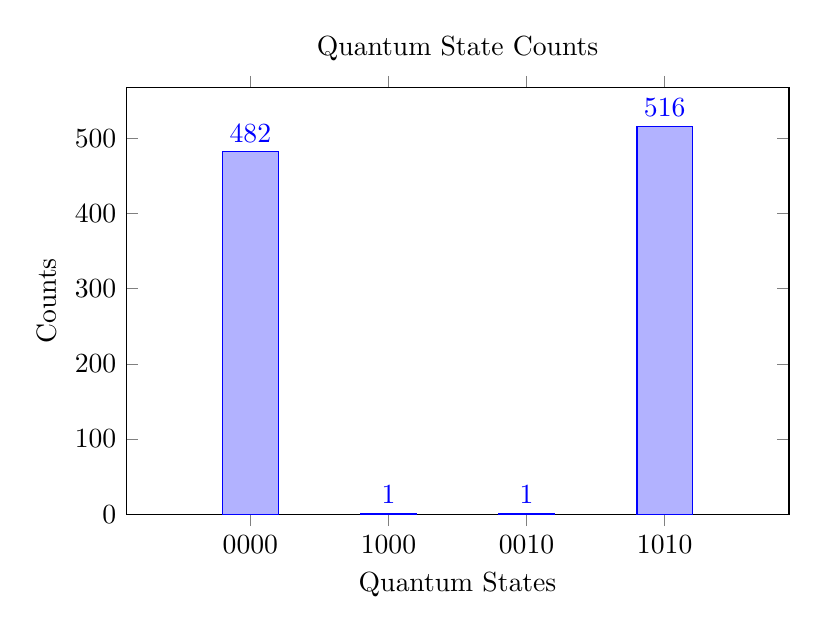
\begin{tikzpicture}
        \begin{axis}[
            ybar,
            symbolic x coords={0000, 1000, 0010, 1010},
            xtick=data,
            xlabel={Quantum States},
            ylabel={Counts},
            ymin=0,
            bar width=20pt,
            width=10cm,
            height=7cm,
            nodes near coords,
            nodes near coords align={vertical},
            enlarge x limits=0.3,
            title={Quantum State Counts}
        ]
        \addplot coordinates {(0000,482) (1000,1) (0010,1) (1010,516) };
        \end{axis}
    \end{tikzpicture}
\end{center}


the OpenQASM 2.0 code for the above qircuit is: 


\begin{verbatim}
qreg q[4];
creg c[4];
h q[0];
h q[1];
cx q[1], q[2];
ry(0.110500) q[2];
cx q[1], q[2];
ry(-0.110500) q[2];
x q[1];
ccx q[0], q[1], q[2];
cx q[0], q[2];
ry(0.000000) q[2];
cx q[0], q[2];
ry(0.000000) q[2];
ccx q[0], q[1], q[2];
cx q[0], q[2];
ry(0.000000) q[2];
cx q[0], q[2];
ry(0.000000) q[2];
x q[0];
ccx q[0], q[1], q[2];
cx q[0], q[2];
ry(-1.511125) q[2];
cx q[0], q[2];
ry(1.511125) q[2];
ccx q[0], q[1], q[2];
cx q[0], q[2];
ry(1.511125) q[2];
cx q[0], q[2];
ry(-1.511125) q[2];
cx q[0], q[3];
h q[1];
measure q[1] -> c[1];
measure q[3] -> c[3];
\end{verbatim}
\end{document}